
\begin{table}[htbp]
\centering
\caption{Persona Suplementar}
\label{tab:Table_persona3}
\small
\begin{tabular}{| m{0.25\textwidth} m{0.65\textwidth}|}
\hline \multicolumn{2}{|c|}{\textbf{Identidade}} \\ \hline
& \\

\begin{center} 
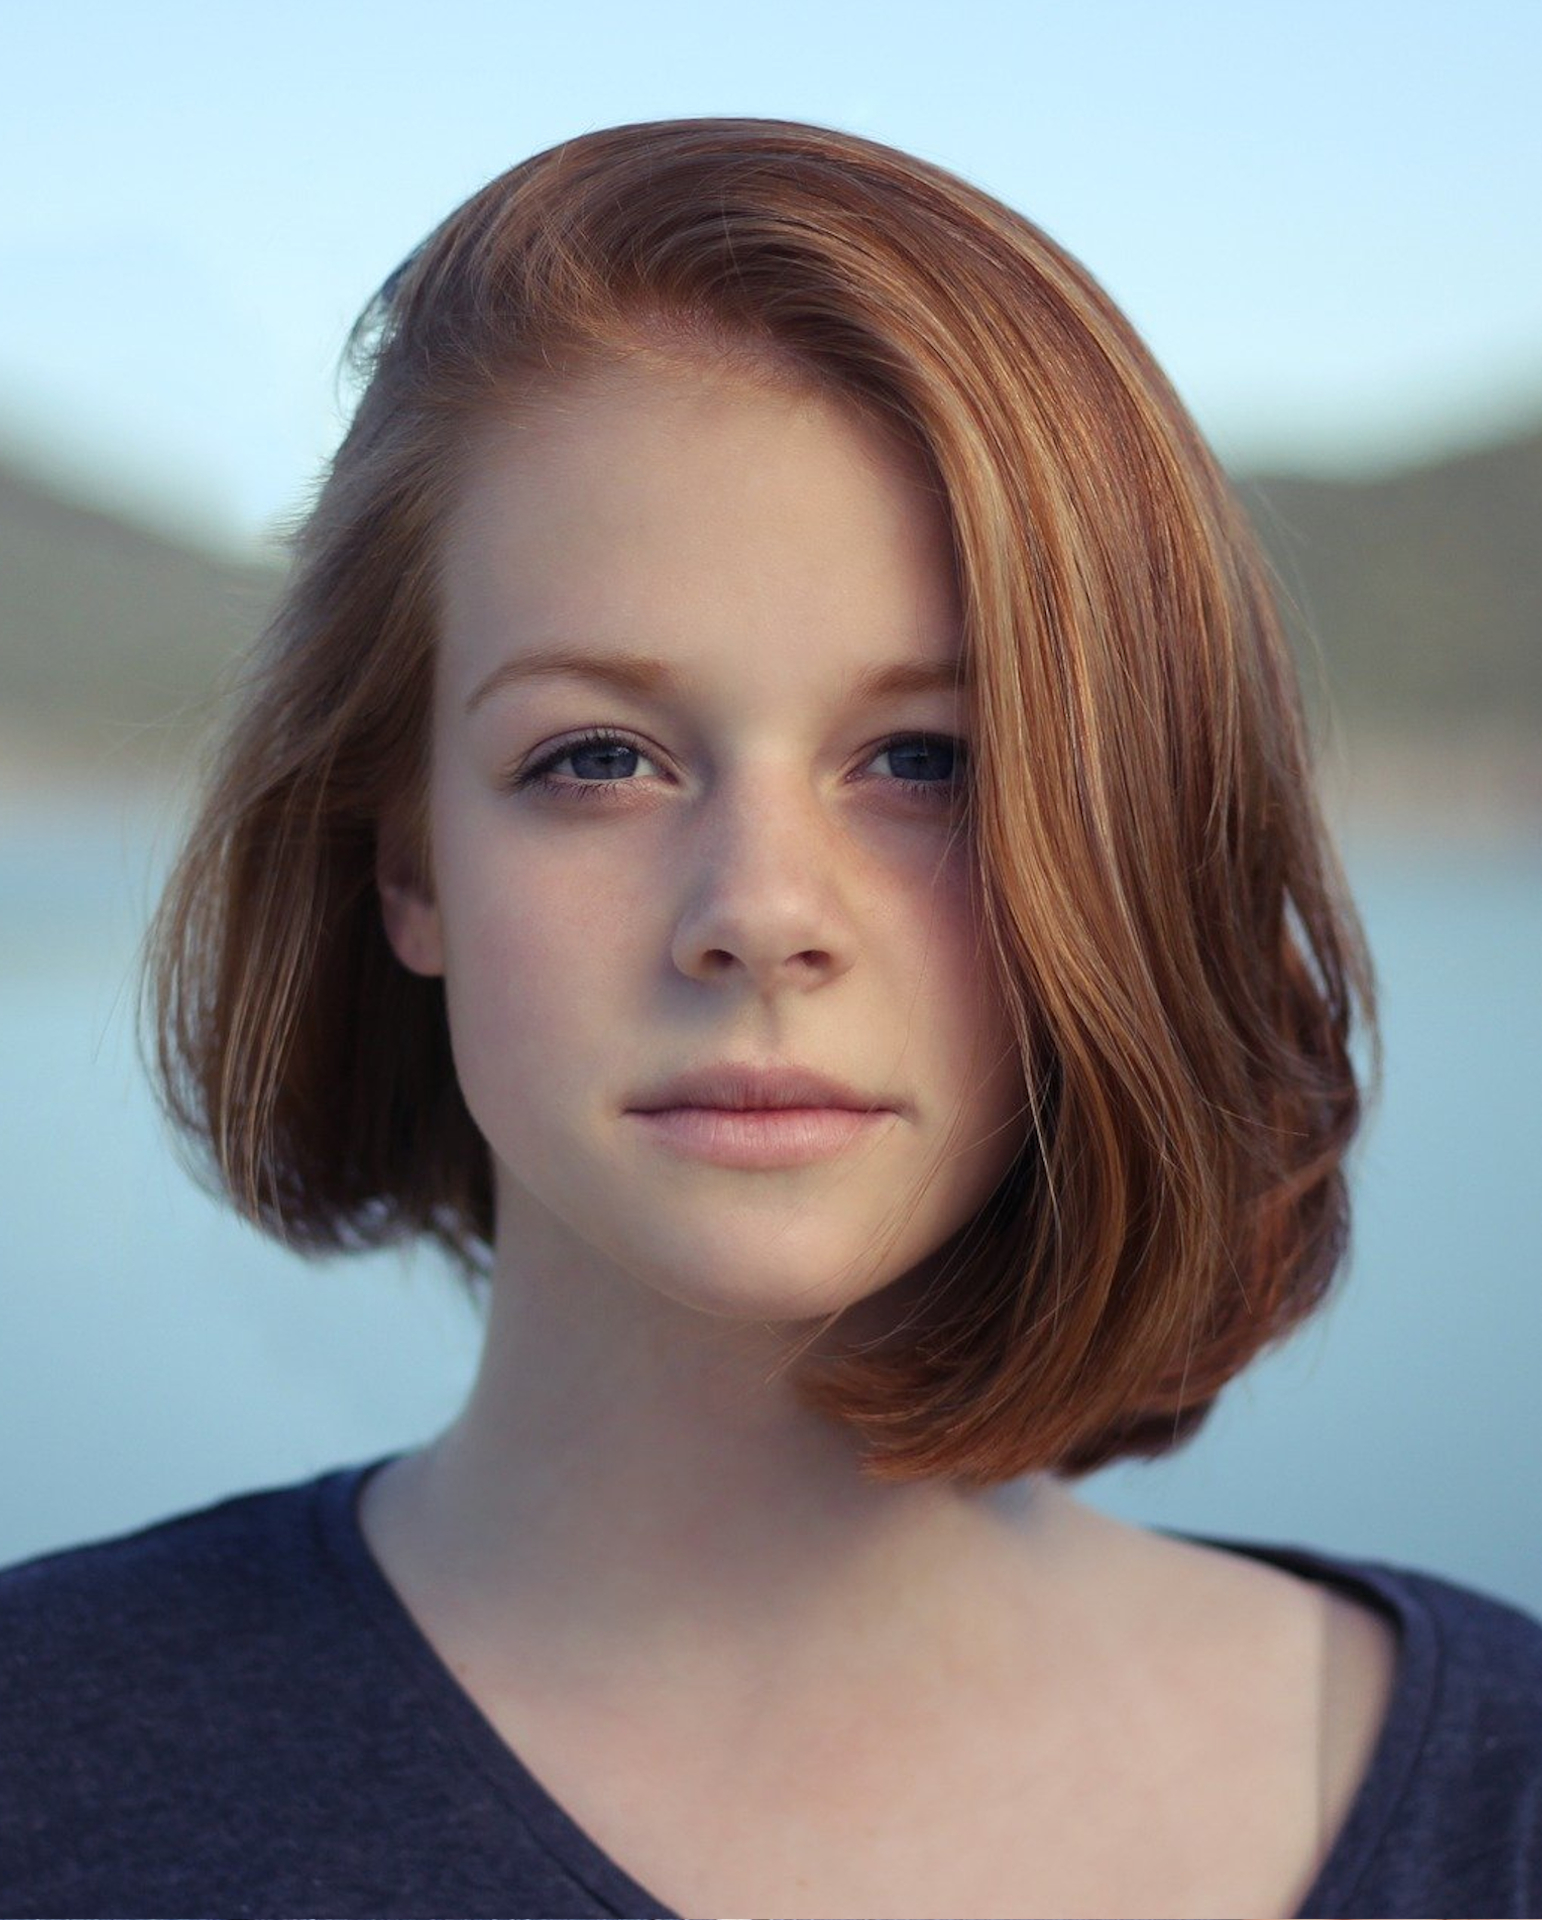
\includegraphics[scale=0.06]{figuras/personas/girl-919048_1920.jpg}
Fonte: Pixabay\tablefootnote{https://pixabay.com/photos/girl-portrait-hairstyle-redhead-919048/}
\end{center} 

&

\textbf{Nome: }  Natália Figueiredo

\textbf{Idade:} 23 anos

\textbf{Ocupação:} Estudante de Engenharia de Software na UnB, Faculdade do Gama.

\\ \hline


\multicolumn{2}{|c|}{\textbf{Descrição}} \\ \hline
\multicolumn{2}{|p{15cm}|}{
    \begin{tabular}[c]{@{}l@{}}\\
        Nunca joguei jogos educacionais, pois não conheci nenhum que tinha o propósito de\\ ensinar o que eu desejava. No caso se eu encontrasse um jogo o qual eu pudesse aprender\\ um conteúdo novo e pudesse revisá-lo quando necessário seria interessante. Estou fazendo\\ a disciplina de IHC e desejaria utilizar um jogo que me ajudasse a aprender o conteúdo,\\ pois não tenho muito conhecimento em relação a elaboração de design de interfaces e o\\ pouco que tenho foi somente a partir da disciplina de IHC.\\
        \\
        Geralmente quando vou estudar ou sanar alguma dúvida que tenho sobre o conteúdo eu\\ pesquiso na internet. Em ocasiões bem específicas eu assisto vídeo aulas e também\\ utilizo do material disponibilizado pelo professor. \\
        \\
        Acho que um jogo para se estudar teria de ter um \textbf{design simples}, uma lógica de jogo e\\ \textbf{regras fáceis} de se lembrar. O jogo não deveria ser muito \textbf{difícil}, sendo que o objetivo\\ com ele é aprender. Talvez \textbf{recompensas} e \textbf{mensagens} evidenciando meu progresso\\ seriam interessantes.\\
        \\
        Ao jogar, espero encontrar \textbf{desafios} não muito difíceis, mas que despertem minha\\ \textbf{atenção}. Seria bom, perceber logo de início que o jogo traz um \textbf{conteúdo relevante} e \\que vou \textbf{conseguir aprendê-lo}. E por fim não seria nada ruim sentir \textbf{prazer} em \\aprender e ainda me \textbf{divertir}.\\
        \\
    \end{tabular}
} \\ \hline
\end{tabular}
\end{table}
\newpage